\documentclass[usegeometry=true]{scrartcl}
\usepackage[ngerman]{babel}
\usepackage[T1]{fontenc}
\usepackage{lmodern}
\usepackage[utf8]{inputenc}
\usepackage{hyperref}
\usepackage{amssymb}
\usepackage{graphicx}
% Dimensionen bitte nicht ändern. 
\usepackage[left=2cm, right=2cm, top=2cm, bottom=2cm, bindingoffset=1cm, includeheadfoot]{geometry}
%Zeilenabstand bitte nicht ändern
\usepackage[onehalfspacing]{setspace}


\bibliographystyle{unsrt}

\begin{document}
% ----------------------------------------------------------------------------
\subject{Projektbericht zum Modul Information Retrieval und Visualisierung Sommersemester 2021}

\title{Bike Buyers 1000}
%\subtitle{Untertitel}% optional
\author{Floyd Spuhler}% obligatorisch
\date{10.09.2021}
\maketitle% verwendet die zuvor gemachte Angaben zur Gestaltung eines Titels
% ----------------------------------------------------------------------------
% Inhaltsverzeichnis:
\newpage
\tableofcontents
% ----------------------------------------------------------------------------
% Gliederung und Text:
\newpage
\section{Einleitung}
Durch das wachsende Umweltbewusstsein in der Bevölkerung rückt besonders das Fahrrad als klimaneutrales Verkehrsmittel in den Fokus \cite{Marquart.2021}. Bereits 2019 betrug der Gesamtbestand an Fahrrädern in Deutschland fast 76 Millionen \cite{Kords.26.06.2020,Statista.25.08.2021}. Die anhaltende Covid-19 Krise verstärkt den zunehmenden Fahrrad-Boom für die Freizeitgestaltung und den Pendelverkehr \cite{Platter.2020}. Gründe hierfür liegen beispielsweise bei der Sportmöglichkeit als Ausgleich zu geschlossenen Sportstätten, sowie im Individualverkehr für das Einhalten der Abstandregeln als Alternative zum Nahverkehr. Dabei wird sich häufig für das Fahrrad anstelle des Autos entschieden. \cite{Kollner.30.12.2020,Thomannbusse.24.11.2020}.Durch die Krise bedingte Lieferverzögerungen und Knappheiten führen zu einer hohen Nachfrage und steigenden Preisen. Auch wärmere Winter begünstigen eine längere Fahrradsaison und sorgen dadurch zusätzlich für Lieferengpässe \cite{tagesschau.11.03.2021}. Neuentwicklungen wie E-Bikes werden immer beliebter, was sich an der Gesamtabsatzbeteiligung im Jahr 2020 von 38,7\% in Deutschland bemerkbar macht \cite{tagesschau.11.03.2021}. 
In der Schweiz ist das Fahrrad nicht zuletzt durch den staatlich geförderten Ausbau von Fahrradspuren zum beliebtesten Verkehrsmittel geworden \cite{Platter.2020}.
Somit stellt diese rasante Entwicklung die Fahrradbranche vor Herausforderungen, die Kundenwünsche richtig umzusetzen. Unübersichtliche Lieferententermine und der Onlinehandel erschweren die Kundenbeziehung. Diese Arbeit möchte diese Probleme durch gezielte Visualisierung von Kundendaten zum Thema Fahrradkauf für verschiedene Branchenbereiche lösen.Im Rahmen dieser Arbeit wird zur Veranschaulichung auf  Visualisierungstechniken wie den Scatterplot, Parallele Koordinaten und das Baumdiagramm zurückgegriffen. 

Diese Arbeit liefert Erkenntnisse in Bezug auf die Zusammenhänge verschiedener Kundendaten, die zu Fahrradkäufen führen können, beantwortet Fragen bezogen auf infrastrukturelle Besonderheiten durch Datenstrukturierung und lässt Anwendende über die Interaktion mit den Visualisierungen weitere Trends und dadurch einen Mehrwert für Ihren Geschäftsbereich ableiten. 


\subsection{Anwendungshintergrund}


Diese Forschungsarbeit bereitet Informationen auf, die interessante Einblicke in das Kaufverhalten von Fahrrad-Kunden geben. So lassen sich anhand von Einkommensdaten, dem Alter und dem Bildungshintergrund Kundengruppen ableiten, auf welche in allen Wertschöpfungsebenen eingegangen werden kann. Hersteller müssen beispielsweise die Rahmengröße auf das Alter abstimmen. Einkommensstarke Kunden setzten den Fokus auf hochwertige Materialien (z.B. Carbon)und erwarten dabei technische Innovation, was die aktuelle Kooperation eines Fahrradunternehmens mit dem Premium-Autohersteller Porsche für ein E-Bike zeigt (NTV). Personen die das Fahrrad zum Pendeln nutzen sind eher auf ein Stadt- als ein Mountainbike angewiesen. Anhand der häufigsten Arbeitsentfernung können Bauunternehmen in Innenstädten gezielter Fahrradwege bauen. Diese Anwendungsfelder werden über die drei verschiedenen Visualisierungsanwendungen aufgegriffen. 

Mit einem Scatterplot, bestehend aus X und Y Achse, können Zusammenhänge von Y in Abhängigkeit von X festgestellt werden. Diese Zusammenhänge werden in Form von Punkten, die zwischen beiden Achsen liegen und einen Achsenwert darstellen, visualisiert. Dabei fallen die Beziehungen zwischen den beiden Punkten je nach  Verwendungszweck unterschiedlich stark aus \cite{Yi.16.10.2019,Anscombe.1973,Cleveland.1984}. Der Scatterplot wird für die Daten zu Fahrradkunden als erste Darstellung von Zusammenhängen verwendet. 

Mit der zweiten Visualisierung, Parallelen Koordinaten, können Zusammenhänge multidimensionaler Daten besser als über Punkte dargestellt werden. Punkte werden dabei zu Achsenbeschriftungen und Linien \cite{Inselberg.1990}. Jede betrachtete Variable wird nebeneinander angeordnet. Alle dazugehörigen Datenwerte werden über eine Linie miteinander verbunden \cite{Moustafa.2006}. 

Die vertikalen Achsen sind über Linien miteinander verbunden. Die Auf- und Ab-Bewegungen der Linien zeigen Werteveränderungen auf \cite{Few.2008}. 
Dabei sind die Achsen parallel zueinander angeordnet. Parallele Koordinaten bieten einen guten Datenüberblick. Eine Gefahr stellt allerdings die Überlappung von Linien dar, wenn zu viele Daten verwendet werden \cite{Heinrich.2009}.

Über ein Baumdiagramm lassen sich Daten und deren Beziehungen untereinander anordnen, wodurch eine übersichtliche Datenstruktur entsteht und sich Daten schnell wiederfinden lassen. Die Baumstruktur besteht aus Knoten und Kanten. Zwei Knoten sind jeweils über eine Kante miteinander verbunden. In der Baumstruktur muss ein Knoten vorhanden sein, der keinen Vorgänger hat. Dieser Knoten wird Wurzel genannt. Dessen Folgeknoten werden Nachfolger genannt. Über die Wurzel führen nur azyklische Pfade und zu jedem Knoten nur ein Pfad. Durch die unterschiedlichen Pfade und Verzweigungen der unterschiedlichen Daten entsteht die Baumstruktur \cite{Gumm.2016}. (S. 289) Diese Visualisierungstechnik eignet sich für die übersichtliche Darstellung bestimmter Daten zu Fahrradkäufen, da diese Daten Strukturen aufweisen, die sich zur Hierarchiedarstellung eignen. Im Datensatz sind des Weiteren Abfragen erhoben worden, ob sich eine Person ein Fahrrad gekauft hat oder nicht. Dadurch lässt sich der Datensatz als Erstes aufteilen. Des Weiteren sollen globale Unterschiede dargestellt werden, um auf territoriale Umfelder eingehen zu können. Ein weiter Faktor ist die Pendeldistanz vom Wohnsitz der Befragten zur Arbeit, welche verschiedene Antwortmöglichkeiten zulässt. All diese Faktoren können kombiniert in die Baumhierarchie übertragen werden.   
\subsection{Zielgruppen}
Dieser Forschungsbericht richtet sich vor allem an die Anbieterseite auf den B2C Fahrradmarkt. Auf der Anbieterseite sind alle in der Lieferkette vorhandenen Unternehmensbrachen betroffen. Die Hersteller haben mit dem Materialmangel zu kämpfen.Den Fahrradverkäufern macht der Onlinehandel Konkurrenz und auch Bauunternehmen, die Fahrradspuren bauen haben mit Rohstoffmangel Probleme.  Hierzu lassen sich drei Hauptzielgruppen, neben Fahrradinteressierten, herausfiltern, an welche sich dieser Visualisierungsbericht richtet.
\begin{itemize}
 \item \textbf{Fahrradhersteller}: 
 \newline Fahrradhersteller benötigen besonders wegen der Materialknappheit spezifische Informationen zu den personenbezogenen Merkmalen potenzieller Kunden, wie z.B. Größe, Alter, Einkommen um einen Fahrradrahmen mit entsprechend wertigen / nicht wertigen Materialien für eine Verwendungszweck (z.B. Mountainbike, Stadtrad)herzustellen 
 Für Fahrradhersteller sind Informationen zum Alter der Kundengruppe für Rahmengröße, Fahrradart, sowie zum Einkommen in Hinblick auf die Auswahl der Materialien und deren Qualität wichtig. 
 \item \textbf{Fahrradhandel}:
 \newline Für Fahrradverkäufer spielt vor allem der Verwendungszweck des potenziellen Kunden eine übergeordnete Rolle beim Fahrradkauf. Die Wahl des richtigen Modells unterscheidet sich für die Freizeit (Mountainbike) mit weiten Distanzen vom Gebrauch für die Stadt mit geringeren Distanzen (Stadtrad). Für weitere Distanzen eignen sich Mountainbikes besser als für die Fahrt in ebenerdigem Terrain, wie asphaltierten Straßen. für Stadträder. Optimalerweise betreibt diese Zielgruppe einen eigenen Onlineshop zum Fahrradvertrieb und benötigt Informationen für die zielgerichtete Kundengruppenwerbung (ggf. Verweis einbauen?). 

 \item \textbf{Bauunternehmen mit dem Fokus auf Fahrradinfrastruktur}:
 \newline Auch für Unternehmen aus der Baubranche mit dem Fokus auf die Infrastruktur für Fahrradwege ist diese Arbeit eine geeignete Anlaufstelle für Informationen zum Einsatz des Fahrrads in Bezug auf den Arbeitsweg. Daten zu Pendlerwegen müssen für diese Zielgruppe besonders aufgegliedert vorliegen, da Bauunternehmen somit Informationen über die benötigten Distanzen neuer Fahrradwege erhalten und besonders in Städten nur begrenzt Raum zur Verfügung haben. Dadurch muss der EInsatz von Baumaschinen beonsders abgewogen werden. 
 
\end{itemize}

Dieser Visualisierungsbericht ermöglicht es den oben genannten Unternehmen eine bessere Kundenmarktsegmentierung zu betreiben.  Kurzfristig können durch die Ergebnisse dieses Berichtes Ressourcen sparsam eingesetzt werden (v.a. Hersteller, Baubranche). Langfristig können besonders Fahradhändler von diesem Bericht profitieren, da sie durch die personenbezogenen Daten optimale Kundenakquise / Kundenberatung garantieren können und anhand von Einkommensparametern Preise bestmöglich bilden können. 



\subsection{Überblick und Beiträge}
Die durch Kaggle bereitgestellten Daten bestehen aus demographischen Kundeninformationen, wie Alter, Geschlecht, Familienstand etc.  Diese Daten werden über die drei Visualisierungstechniken Scatterplot, Parallele Koordinaten und Baumhierarchie abgebildet, um den in 1.2 angesprochenen Zielgruppen einen Überblick in diese Kundendaten zu vermitteln.Über den Scatterplot können jeweils zwei Dateneigenschaften einander gegenübergestellt werden. Bei der Anwendung kann über Buttons selbst ausgewählt werden, welche beiden Eigenschaften angezeigt werden sollen. Mit den parallelen Koordinaten haben Interessenten die Möglichkeit über vertikale Achsen Werte miteinander zu vergleichen. Buttons ermöglichen hierbei die dynamische Achsenverschiebung. Die Baumhierarchie lässt die Daten anhand wesentlicher Eigenschaften in verschiedenen Ebenen darstellen. 

\section{Daten}
Die diesem Projektbericht zugrundeliegenden Rohdaten entstammen einem Datensatz des " Kaggle" -Account von Heeral Dedhia \cite{Dedhia.22.09.2020}, welche Antworten von 1.000 NutzerInnen zum Thema Fahrradkauf bereitstellt. Die Nutzerin hat diese Daten zuletzt im Jahresverlauf 2020 erweitert. Datum- und Erhebungsform sind hierbei unbekannt. In dieser aktuellsten Version liegen 13 verschiedene Attribute zu den 1000 befragten Personen vor. Die Nutzerin hat zwei verschiedene Datensätze bereitgestellt, die sich lediglich durch NA-Werte unterscheiden. Um bei einer Datenvorverarbeitung keine Daten zu vergessen und die Funktionsfähigkeit des Elm CSV-Decoders zu gewährleisten, stellt die bereinigte Datei "bikebuyersclean.csv" die Grundlage für dieses Visualisierungsprojekt dar (ToDo: Kaggle Seite zitieren). 

zu allen befragten personen wurde eine eindeugige ID vergeben, welche ein INT-Typ ist. Zur quantifizierung der Baumhierarchie wurde diese Tabellenspalte für die dritte Visualiserung übernommen. Die nächsten beiden Spalten "Marital Status" , "Gender" und "Children" und "Age" als Int geben als String-Datentyp Aufschluss über den sozialen  Familienstand und Geschlecht der befragten Person. Die Spalten "Income", "Education" , "Occupation" geben Auffschluss über die berufliche Karriere. In Verbindung mit den Spalten "HomeOwner" und "Cars" lässt sich der Status der Person interpretieren. Das Attribut "Commute Distance" gibt Aufschluss über die Distanz zur Arbeit" dient der Befragung zur Entfernung zwischen Wohnort und Arbeitsstätte, wodurch wertvolle Informationen zwischen Cars, Bikes und co gewonnen werden können. Durch purchasedBike und Region können diese Daten weiter voneinander unterschieden oder für einen globalen Einblcik als ganzes betrachtet werden. 

Die Daten eignen sich besonders für Analysten von Fahrradunternehmen, die beispielsweise einen Online-Fahhrad-Shop betreiben wollen. Hierdurch erhalten sie eine Grundlage über mögliche Kundengruppen, wodurch wertvolle Informationen, wie die Arbeitsentferung vorhanden sind und sich insbesondere in der zukünftigen Infrastruktur von Großstädten bemerkbar machen werden. Auch in Hinblick auf die anhaltende covid-19 Krise und den sicheren Aspekt des Individualverkehrs bietet eiun Fahrad auf kurze bis mittlere Distanz eine umweltschonende und kostengünstige Alternative zum Auto. 
Diese Informationen in Verbindlung mit dem Alter, Einkommen und Beruf können individuelle Kundengruppen angesprochen werden. 

Um eine geeignete Überblicksmöglichkeit über diese potenziellen Kundengruppen zu schaffen, musste der dafür notwendige Datensatz für die Baumhierarchie angepasst werden. 

\subsection{Technische Bereitstellung der Daten}


Die dem Kaggle Account (hier Ztat) entstammenden, bereinigten Rohdaten in der Datei "bike buyers clean.csv" wurden in das Github Repository des Autors hochgeladen. Diese ist im Ordner "Daten zum Laden" abgelegt. Für die beiden Elm Dateien "Scatterplot.elm" und "Parallele Koordinaten.elm" wurden die vollständigen Daten der durch Kaggle bereitgestellten Datei als String in die jeweiligen ELM Dateien geladen. Dieses Vorgehen ermöglicht die dauerhafte Visualisierungdsdarstellung und ist unabhängig von Linkveränderungen. Das für die Baumhierarchie notwenige JSON-Format wird im Ordner "JSON" durch die Datei "DatenvorverarbeitungohneCarWolrdwide.json" bereitgestellt und über einen Link in die entsprechende Elm-Datei "Baumhierarchie.elm" geladen. 

Der zugrundeliegende Datensatz wurde um keine zusätzlichen Daten erweitert. Die Daten bilden eine gute Verteilung in verschiedenen Regionen ab, sind ausgewogen verteilt und bieten eine vielzahl an Informationen, mit denen Fahrradhersteller / Verkäufer wie Onlineshiops gezielt Kundengruppen ansprechen können. 
\subsection{Datenvorverarbeitung}

Um die CSV Daten in den jeweiligen ELM Programme zu verwenden war für die Dateien "Scatterplot.elm" und "ParalleleKoordinaten.elm" keine Datenvorverarbeitung notwendig. Die Rohdaten wurden in der jeweiligen Datei als String hinzugefügt und entsprechend decodiert. 
Die Datei "Visualisierung3 Vorverarbeitung.xlsx" zeigt das Ergebnis, dass aus dem CSV-String der Rohdatei einzelne Excel Spalten gemacht wurden. Für die Datrstellungsziele der Baumhierarchie sind die Spalten ID, Cars, Commute Distance, Region und Purchased Bike notwenig. Die übrigen Datenattribute wurden für die Vorerarbeitung für die JSON-Transformation entfernt.  Die wichigen Attribute sind in der Datei "Visualsierung3 Vorverarbeitung.csv" enthalten. Die Spalte ID wurde für die letzte Hierarchieebene in eine neue Spalte zusammen mit "data id " übertragen, damit die Daten vom ELm Json Decoder erkannt werden. Dies erfolgte mit dem Excelbefehl "Verketten(...)". Anschließend wurden die Daten ausgewählt, welche 0 Autos aufweisen, damit der Effekt zwischen Fahrradkäufern und Nicht-Käufern und deren Pendler-Distanz vergleichbar wird. Für die JSOn Atei wurde die Länderliste aus der Übung als Vorlage für den Syntax genommen. Dabei wurden alle Länder raus gelöscht. In den Syntax wurden die Daten übertragen und um die Ebene mit den IDs aus der CSV- Datei erweitert. 
\paragraph{Vorverarbeitung:} Die Vorverarbeitung erfolgt im filtern leerer Felder

\section{Visualisierungen}
\subsection{Analyse der Anwendungsaufgaben}
Über den Scatterplot erhält besonders die Zielgruppe der Fahrradhersteller wichtige Informationen auf einen Blick, die bei der Produktion unterstützen können. 
Mit den Paralleln Koordinaten können die Zusammenhaänge der Zahlenwerte aus dem Datensatz besser untersucht werden. Die Röntgendarstellung ermöglicht es, Überschneidungsmuster gut zu erkennen. Hierdurch haben vor allem neue Fahradhandelsgeschäfte (auch mit Onlineshop) die Möglichkeit Ihren Kundengruppen zielgrerichteter Fahrräder anzubieten, wodurch die Value Proporsition un d die mit dem Fahrrradkauf verbundenen, positiven Erinnerungen stärker hervorgerufen werden können. 

\subsection{Anforderungen an die Visualisierungen}
Im ersten Kapitel wurde die eingehende Motivation beschrieben, den verschiedenen Zielgruppen bestmögliche Anhaltspunkte zu finden, um die Fahrradkungengruppe nachhaltig an die jeweilige Unternehmensbranche zu binden. Die Designs müssen die angesprochene Übersichtlichkeit einhalten. Des Weiteren liegt ihr Wertversrpechen für die Zielgruppe im Aufzeigen von Zusammenhängen und vereinfachen von Datenmengen. Dabei müssen die Visualisierungen besondere Merkmale gut hervorheben, was auf Grund der Datensatzgröße (n=1000) eine Herausforderung darstellt. 
\subsection{Präsentation der Visualisierungen}
In diesem Abschnitt werden die drei dem Projektbericht zugrunde liegenden Visualisierungen, der Scatterplot, Parallele Koordinaten und die Baumhierarchie. 
\subsubsection{Visualisierung Eins}
Für die erste Darstellung wurde der Scatterplot gewählt. Dessen einfache Grundfunktionen bieten eine gute Einleitung in die Visualiserung der Fahrradwerte. Die in der Einleitung beschriebenen Merkmale, wie die gegenüberstellung der X und Y Achse erfolgt über die Datenwerte Alter auf der X Achse und in dieser Abbildung über Einkommen. Anwendende haben darüber hinaus die Möglichkeit, über die oben gelegenen Buttons die Y-Achse des Scatterplots dynamisch anzupassen. Dabei können Einkommen, die Kinder- und Autoanzahl des Datensatzes in Abhängigkeit des Alters dargestellt werden und Die Punkte stellen jeweils einen koordinatenpunkt aus dem BikeBuyers Index dar. Um die Zielgruppe mit Zusatzinformationen zu versorgen können beim Hovern mit der Maus über die Punkte neben dem exakten Einkommen auch Informationen ob ein Fahrradkauf getätigt wurde und welcher Berufsgruppe die befragte Person angehört, eingeholt werden. Die Wahl den Beruf beim Hovern über die punkte  anzuzeigen, lässt sich damit begründen, dass String-Werte nicht in den Achsen dargestellt werden können. 
\begin{figure}[h]
\begin{center}
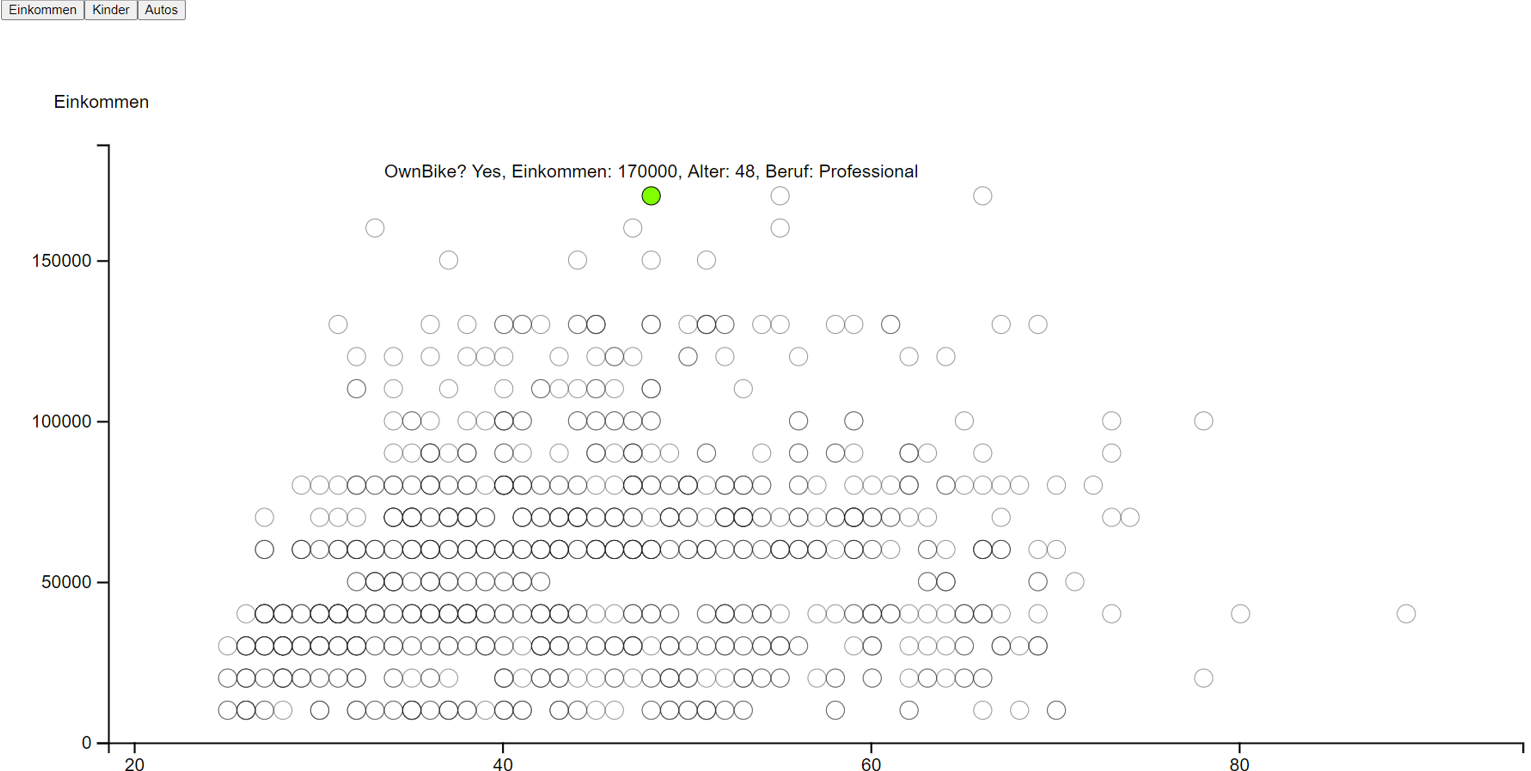
\includegraphics[width=16cm]{Bilder/ScatterplotV1.png}
\caption{Scatterplot für Bike Buyers, Quelle: Eigene Darstellung}
\end{center}
\end{figure}
Die in der Einleitung herausgearbeiteten Scatterplot-Anforderungen können wie in Abbildung 1 entnehmbar, umgesetzt werden. Die beliebige Y-Achsenverändrung erweitert die Anforderungen darhingehend, das Anwendendende den Darstellungs-Inhalt und somit bestinmnte Schwerpunkte selbt setzten können. Stärker sichtbare Punkte bedeuten, dass  Angaben der befragten Personen in diesen Punkten stärker übereinstimmen, als in helleren Punkten.   
Eine Alternative zum Scatterplot stellen die Zeitreihendiagramme dar, wodurch Zeitliche Verläufe anhand vorbestimmter Faktoren als Linien dargestellt werden. Da der vorliegende Datensatz keine zeitlichen Ausprägungen hat, welche chronologisch dargestellt werden könnten, sondern zeitlich unabhängige Werte beinhaltet wurde der Scatterplot als zweidimeinsionale Datenvisualiserung gewählt.


\subsubsection{Visualisierung Zwei}
Mit der zweiten Visualisierung, den Parallelen Koordinaten, können Im Gegensatz zum Scatterplot mehrdimensionale Zahlenwerte gleichzeitig, über vertikale Achsen ohne X Achse dargestellt werden.
Für den Datensatz der bikeBuyers ergibt sich hierdurch den Vorteil, gleichzeitig alle relevanten Zahlenwerte in einer Visualisierung darzustellen, was sich in Abbildung 2 bemerkbar macht. Ebenso wie beim Scatterplot haben Anwendende die Möglichkeit die Darstellung über Buttons zu verändern. Durch die Buttons können die Achsen beliebig miteinander vertauscht werden und neue Zusammenhänge, je nach Betrachtungsziel,identifiziert werden. 
\begin{figure}[h]
\begin{center}
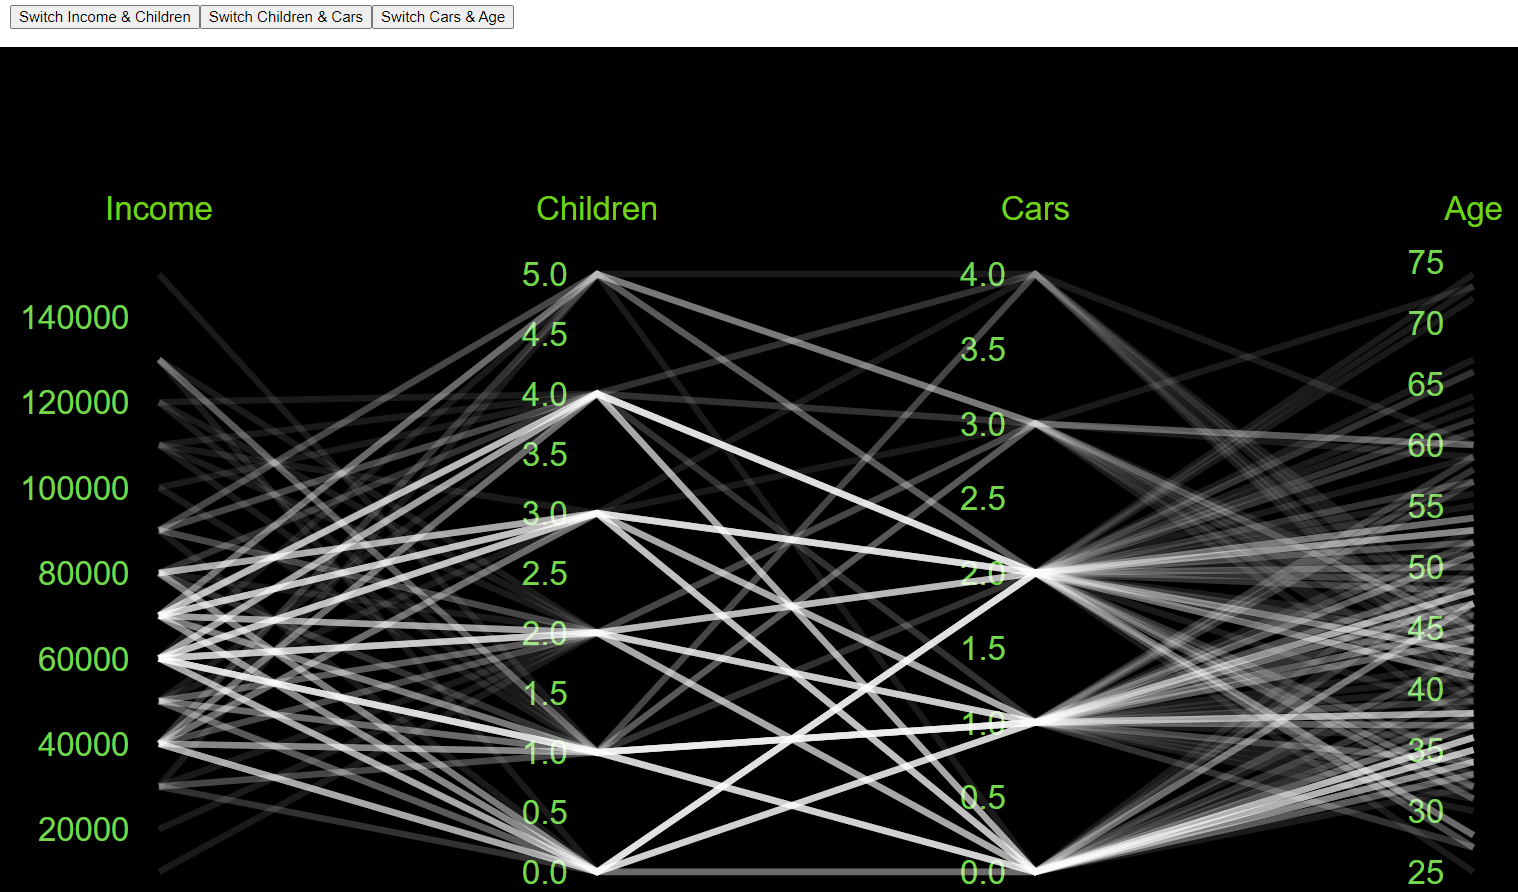
\includegraphics[width=16cm]{Bilder/ParallelCoordsV2.png}
\caption{Parallele Koordinaten für Bike Buyers, Quelle: Eigene Darstellung}
\end{center}
\end{figure}
\newline
Die Abbildung 2 zeigt von links nach rechts den Verlauf eines mehrdimensionalen Punktes beginnend mit dem Einkommen, der Kinder- und Autoanzahl und dem Alter der befragten Person. Der Vorteil im Vergleich zum Scatterplot ist, dass mehrere Zusammenhänge und Auffälligkeiten gleichzeitig erkennbar sind. Im Direktvergleich mit der Darstellung 2 gibt es keine Hoverfunktion, wodurch die Linien individuell nach verfolgbar wären. Durch die Wahl des dunklen Hintergrunds und der hellen Linienfarbe ergibt sich allerdings eine Röntgendarstellung. Durch die Linienüberlappung werden Identifikationsmuster sichtbar, was sich durch die kräftigeren Weißtöne erkennen lässt. Darüber hinaus bietet die durchgängige Achsenbeschriftung gute Anhaltspunkte für den Linienverlauf. Das Vorfiltern nach Region und Fahrradkauf im ELM-Programm verhindert eine "Überdarstellung".  Somit wurden nicht nur alle Anforderungen gemäß der Theorie richtig abgeleitet, sondern auch die Gefahr der "Übervisualisierung" erkannt und verhindert.
Neben Parallelen Koordinaten gibt es weitere Visualisierungsmöglichkeiten mehrdimensionaler Daten. Da Scatterplots, am besten für zweidimensionale Daten geeignet, bereits verwendet wurden, stellen Projektion und Sektion, Sternkoordinaten, K-Means und Datentinte eine Alternative zu Parallelen Koordinaten dar. Mit Projektionen und Sektionen soll der mehrdimensionale Raum abgebildet werden. EIne hierfür anfallende hohe Anzahl an benötigten Darstellungen kommt in Bezug auf die Übersichtlichkeit und Anschaulichkeit für die Zielgruppen nicht in Frage. Mit Sternenkoordinaten können mehrdimensionale Daten in 2D oder in 3D abgebilfet werden. Der Name ist charakteristisch für die Achsenanordung. Auf Grund der ungewöhnlichen Erscheinung und der besseren intuitiven Nachvollziehbarkeit der Fahrradkäuferdaten wurde auf die Parallelen Koordinaten zurückgegriffen. Die Visualisierungstechniken K-Means und Datentinte fokussieren die Visualiserung durch Vorabberechnungen auf wenige Kerngedanken und verhindern somit einen Überblick über eine breitere Sichtweise, welche für alle Zielgruppen anvisiert wurde. Aus diesen Gründen wurde die Parallele Korrdinaten Visualiserung gewählt. 

\subsubsection{Visualisierung Drei}
Als dritte Visualiserungstechnik wurde die Baumhierarchie ausgewählt. Diese stellt ein klassisches Baumdiagramm, wie in der Theorie beschrieben dar, durch welches die Fahrradkäuferdaten in eine Hierarchie gebracht werden. Die Knoten stellen hierbei Entscheidungsmöglichkeiten dar, welche durch die Linien miteinander verbunden werden. Die erste Unterscheidung besteht beim Fahrradkauf. Hierbei werden die Angaben in Ja oder Nein unterteilt. Anschließend erfolgt die Unterteilung nach den Regionen der befragten Personen. Die letzte Verweigung stellt die Pendlerdistan vom Wohnort zur Arbeit dar. 
\begin{figure}[h]
\begin{center}
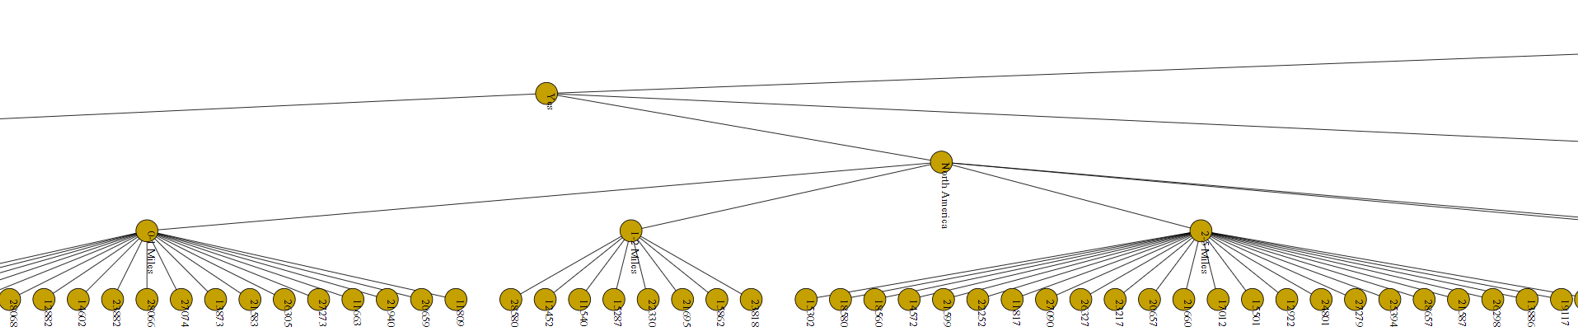
\includegraphics[width=16cm]{Bilder/Baumhierarchie.png}
\caption{Ausschnitt aus der Baumhierarchie für Bike Buyers, Quelle: Eigene Darstellung}
\end{center}
\end{figure}
\newline
Die Abbildung 3 zeigt einen Ausschnitt aus der umfangreichen Baumdarstellung. Hierbei lassen sich die eingefärbten Knoten gut unterscheiden. Im Vergleich zu den beiden vorangegangenen Visualiserungen wurde auf eine Interaktionsmöglichkeit verzichtet. Die angeleiteten Baumhierarchie-Bedingungen, nämlich die übersichtliche Darstellung und Einteilung in Gruppen konnte umgesetzt werden. Trotz Vorfilterung der Parameter, dass die befragten Personen keine Autos besitze, ist die Baumstruktur sehr umfangreich, was zu Überlappungen in der HTML-Darstellungen in der letzten Verzweigung geführt hat. Aus diesem Grund wurde auf weitere Parameter (wie Beruf, oder Bildungsgrad) verzichtet, da diese teilweise über den Scatterplot gezeigt werden. Neben der Möglichkeit die dritte Visualisierung als Baum darzustellen, gibt es weitere Kategorien, die die Darstellung komplexer machen. Hierunter fallen verschiedene Graphenanwendungen, die Mehrfachzuweisungen auf Knoten ermöglichen. Auf Grund der Zielsetzung, abgestuft aufzeigen, welche Pendlerdistanzen auftreten, wurde auf eine komplexere Darstellungsmethode verzichtet. 
\subsection{Interaktion}
Für die Visualisierungen Scatterplot und Parallele Koordinaten wurden zwei verschiedene Interaktionsmöglichkeiten in den jeweils zugrunde liegenden Code integriert. 

Bei der Visualiserung des Scatterplots haben Anwendende die Option, die Gegenüberstellung des Alters auf der X Achse mit einem beliebig verfügbaren Zahlenwert des Bike-Buyers-Datensatzes auf der Y-Achse  über das Klicken auf die verschiedenen Buttons anzeigen zu lassen. Dadurch kann der Fokus individuell auf bestimmte Sachverhalte gelegt werden, was insbesondere für Fahrradhersteller und Fahrradhändler interessant ist. Um die eingeschränkte Funktionalität der zweidimensionalen Zahlengegenüberstellung zu erweitern, wurde die Hover-Funktion integriert. Durch das Hovern über den Punkten des aufgespannten Koordinatensystems werden auch String-Werte als Informationen, wie der Beruf ausgegeben. Daneben lassen sich die exakten Datenwerte beim Einkommen anzeigen, welche als Achseneinteilung zu ungenau wären. 

Die zweite Visualsierung, Parallele Koordinaten, bietet Interessenten die Möglichkeit über Buttons die Achsen nach belieben zu verschieben. Je nach Einstellung lassen sich Zusammenhänge des mehrdoímensionalen Punktes hervorheben, was durch eine eindeutigere Überlappung der hellen Linien sichtbar wird. Anwendende werden dadurch ermutigt, selbst die Daten in eine für sie interessante Sichtweise zu bringen. 

Für das Baumdiagramm wurde auf eine Interaktionsmöglichkeit verzichtet, da das Visualsierungsziel über eine Version erfüllt ist. 

Über eine Hauptseite (index.html) kann aus dem Github Repository eine Website dargestellt werden. Dabei wurden die drei Visualiserungen als HTML, hervorgerufen durch  den Terminalbefehl elm make, jeweils verlinkt. Untereinander findet ebenfalls eine Verlinkung statt, sodass eine Interaktion möglich ist. Diese Interaktion ist über Buttons abrufbar. 

\section{Implementierung}
Die Ausgangsbasis für diesen Projektbericht stellen die Programmcodes aus der Übung dar. Für die Scatterplot Visualiserung wurden die im Rahmen der Übungen eins, drei entwickelten Codegerüste als Grundlage verwendet. Für die Parallelen Koordinaten ist die Übung 7 der Ausgangspunkt. Bei der Baumhierarchie galt die Übung 10 als Orientierung. 

Während der frühen Entwicklungsphase zu Beginn des Projektes wurde versucht, mit Hilfe des CSV-Decoders nach dem Vorbild aus Übug 8 die Daten zu laden. Allerdings ist der unübersichtliche Aufbau des Decoders nicht für die Projektarbeit mit den Fahrraddaten geeignet. Hierzu sind weitere Decodr Funktionen notenig, Daten können nicht direkt nach ihren natürlichen Datentypen decodet werden, etc. Bereits nach der ersten Sichtung des Bike-Buyers-1000 Datensatzes wurde überlegt, die Daten als String in das Codeprogramm zu laden. damit verbundene Vorteile wurden im Kapitel 2 aufgeführt. 
Nach intensiver Alternativenrecherche wurden die Programmcoides für den Scatterplot und die Parallelen Koordinaten nach dem Vorbild des CSV-Decoders von Brian Hicks aufgebaut. Dieser besteht aus einer Funktion, welche problemlos Strings, Ints und Floats decodet. Drüber hinaus ist der Decoder explizit für das Decoden eines CSV-Strings geeignet. 

Eine weitere Herausforderung stellt das Übertragen der Codefundamente aus der Übung auf den neuen Sachverhalt mit den Fahrraddaten dar. In der Übung stellt der Datensatz einen für ELM optimal geeignet Datensatz dar, über welchen eigene Datentypen problemlos über "type" definiert werden können und anschließend damit filterungen durchgeführt wrden können. 


Der Code wurde in mehren Phasen erstellt. Nach erfolgreichen Decoder Tests wurden die Daten mit den zugrundeliegenden Funktionen für den Scatterplot verbunden. Komplikationen mit dem Einbinden des Decoders in die main Funktionen konnten gelöst werden. Nach Erweiterung und individueller Anpassung des Codes konnte ein Scatterplot komiliert werden. Hierbei war die Hoverfunktion bereits integriert. Die Überlegte weiterentwicklung mit Buttons konnte über die init model view update Elm-Grundgleiderung umgesetzt werden. 
Wie sieht die Elm-Datenstruktur für das Model aus, in dem die verschiedenen Zustände der Interaktion gespeichert werden können.
Das Vorgehen wurde bei den Parallen Koordinaten ebenfalls angewendet. Nach erfolgreicher Implementierung und Verknüpfung des Decoders, Anpassen / Erweitern der Daten, inklusive neuer Vorfilterung konnte die Darstellung umgesetzt werden. Nach Abwägung der vOR- UND Nachteile der Röntgendarstellung im vergleich zu "normalem" Hintergrund, wurde die Röntegendatrstellung ausgewählt. Die Weiterentwicklung wurde mit dem Ziel umgesetzt, dass sich die Achsen beliebig verschieben lassen. Diese Umsetzung konnte anhand der Übung 7 erreicht werden.
Bei der Visualisierung der Baumhierarchie gab es bis auf die Datenvorverarbeitung keine Probleme mit dem JSON-Decoder und dem verfügbaren Programmcode aus der Übung 10. 
Zu Beginn jeder der drei Elm-Dateien werden die benötigten ELM-Packages importiert, um sie im Programm zu verwenden. Die genaue Aufzählung der Packages ist in der readme zu finden. 
\section{Anwendungsfälle}
Im folgenden werden für die drei Darstellungen in Hinblick auf die Zielgruppe praktische Anwendungsfälle aufgezeigt. 
\subsection{Anwendung Visualisierung Eins}

Grundsätzlich werden über die Hoverfunktion beim Scatterplot wichtige Zusatzinformationen geliefert, die genauer über die Buttons angezeigt werden können. DIe erste Möglichkeit vergleicht das Alter mit dem Einkommen. 

\begin{figure}[h]
\begin{center}
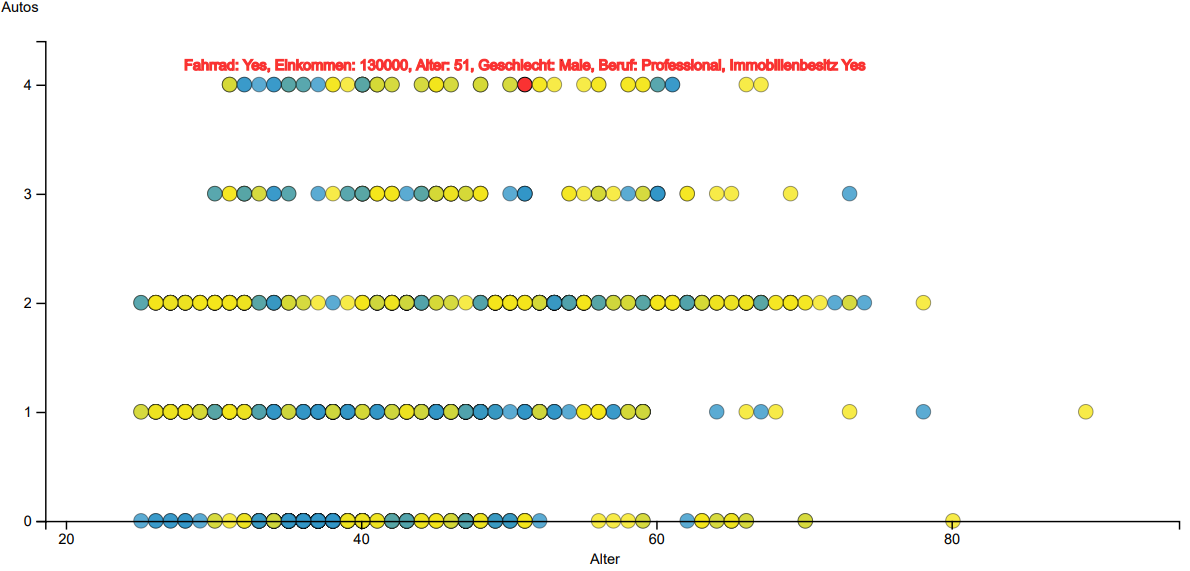
\includegraphics[width=16cm]{Bilder/ScatterplotA1.png}
\caption{Anwendung Scatterplot, Quelle: Eigene Darstellung}
\end{center}
\end{figure}
In der Abbildujg 4 ist ein Scatterplot abgebilkdet, welcher sich besonders für die Zielgruppe des Fahrradhandels richtet. Durch Informationen, ob Kaufinteressierte eines Fahrrads ein Eigenheim besitzen kann auf eine Familie geschlossen werden, welche potenziell Platz für mehrere Fahrräder hat. Durch eine intensivierung der Kundenbeziehung, wie z.B. Rabtte beim Kauf eines zusätzlichen Kiunderfahrrads kann generationenübergreifend Fahrräder verkauft werden. Des weiteren kann aus dem Scatterplot entnommen werden, dass ab einem Alter von 30 Jahren die Kinderanzahl zunimmt und davor überwiegend zwischen 0 und 1 liegt. Mit der Zusatzinformation, ob die kaufinteressierte Person ein Eigenheim besitzt kann aber auch eine potenziell einkommensstarke Kundengruppe eingeordet werden, wodurch höherwertigere fahrräder für verschiedene Verwendungszwecke beworben werden können. Durch die Hover-Anzeige des Einkommens wird ersichtlich, dass Personen mit 4-5 Kindern ein hohes Einkommen aufweisen. 
\newpage

\subsection{Anwendung Visualisierung Zwei}
Die zweite Anwendung stellt die in Abbildung 5 gezeigte umstellung der Achsen dar. Diese ist besonders für Fahrradhersteller geeignet. Im Elm programmcode wurden Daten herausgefiltert, die "nein" zum Fahrradkauf und als region nicht Europe angeben haben. Durch die erste Filterung lässt sich für die Fahrradhersteller besser erkennen, was gemacht werden muss. Die zweite Vorfilterung wurde vorgenaommen, damit der Datensatz auf Grund zu vieler Daten nicht zu unübersichtlich wird. Die meisten Datenwerte sind für die Region North America verfügbar. Danach folgen in Abstufender Reihenfolge "Europe" und "Pacific". Europa wurde auf Grubd des regionalen bezugs und der damit einhergehenden Assoziation für Regionale Bauunternehmen gewählt.
\begin{figure}[h]
\begin{center}
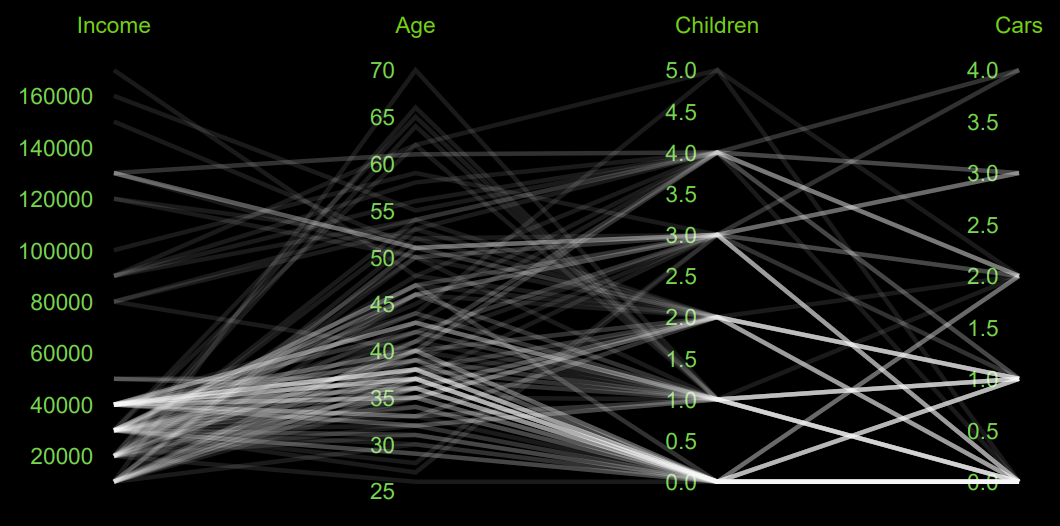
\includegraphics[width=16cm]{Bilder/ParallelCoordsA2.png}
\caption{Anwendung Parallele Koordinaten, Quelle: Eigene Darstellung}
\end{center}
\end{figure}
\newline In dieser Abbildung lässt sich erkennen, dass die höchsten EInkommen in den Altersgruppen zwischen 35 und 55 Jahren generiert werden. In Hinblick auf den Karrieweg vom Berufbeginn und Renteneintritt ist dieser Effekt logisch u erklären. In Hinblick auf das gestell des Fahrrads müssen somit keine Merkmale auf Aufstiegsfreundlichkeit gelegt werden. 
\newpage
\subsection{Anwendung Visualisierung Drei}
\begin{figure}[h]
\begin{center}
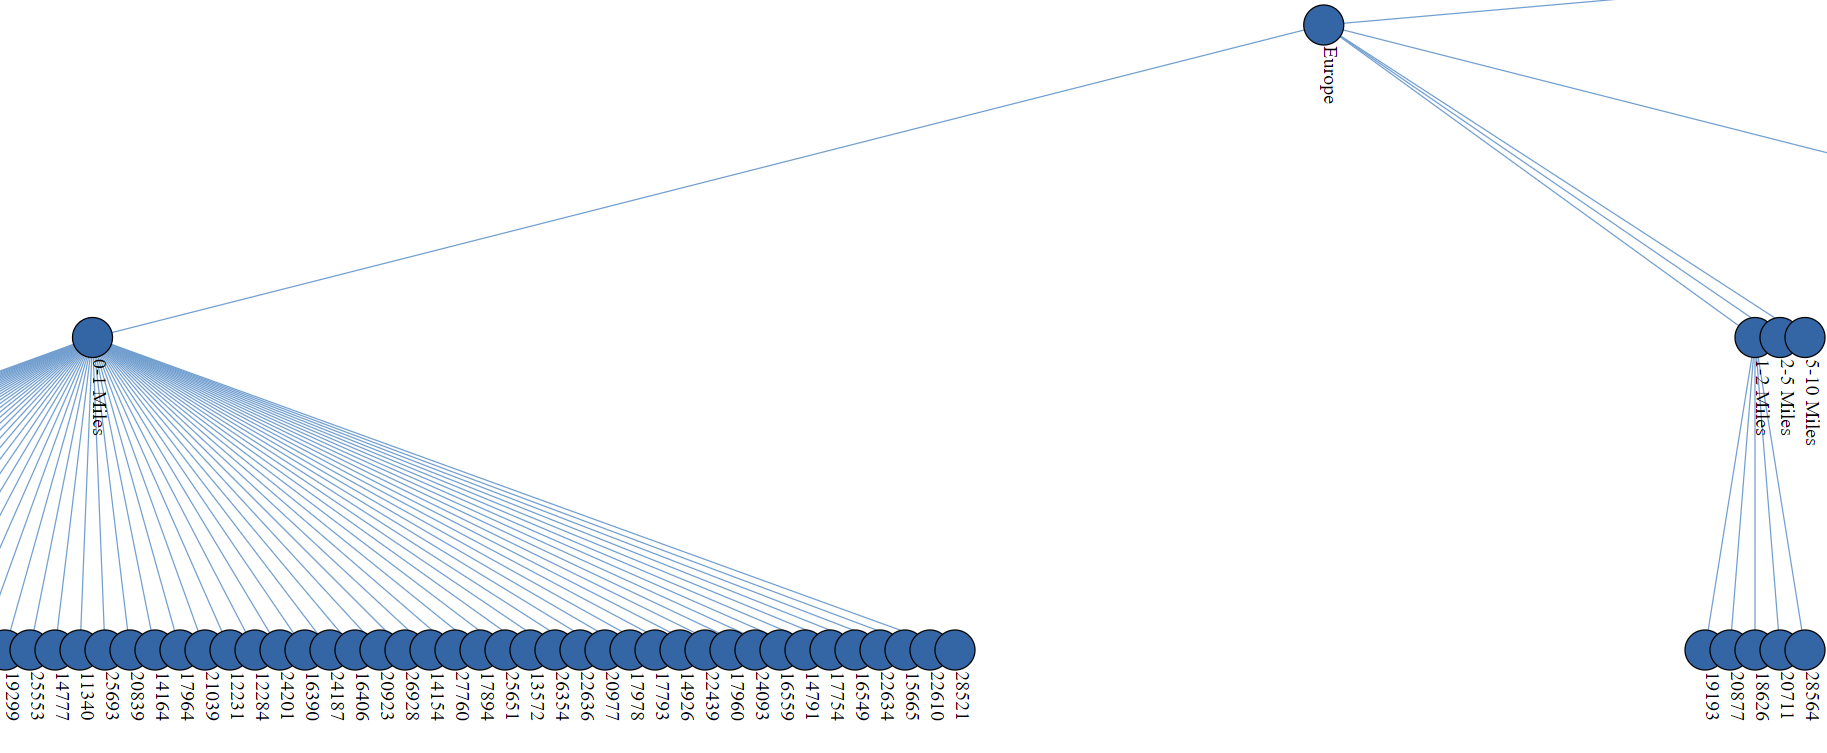
\includegraphics[width=16cm]{Bilder/BaumhierarchieA3.png}
\caption{Anwendung Baumhierarchie, Quelle: Eigene Darstellung}
\end{center}
\end{figure}
Aus der Abbildung 6 geht hervor, dass in Europa von den Fahrradkäufern ohne Auto die überwiegende mehrheit eine geringe Distanz von Zuhause zur Arbeit aufweist. Da diese Distanz für den öffentlichen Nahverkehr zu gering wäre, gleichzeitig aber Distanzen von 1.6 km nicht mehr uzeitsparend zu Fuß zu bewältigen sind, kann davon augegangen werden, dass viele dieser Fahrradkäufer das Fahrrad zur Arbeit verwenden. Auf Grund der kurzen Entfernung ist davon auszugehen, dass die Daten in Großstädten gesammelt wurden. Die Infrastrukut ist hiervon von mehrspurigen Straßen mit vielen kruezungen und Abbiegungen gekennzeichnet. Infrastrukturprogeomme sehehn hierzu vor, dass besonders Fahrradwege besser ausgebaut werden sollen, damit weniger Verkehrsunfälle mit Fahrrädern passieren. Gerade deshalb ist dieser Ausschnitt aus der baumghierarchie für in Frage kommende Bauunternehmen spannend. Daran lässt sich erkennen, dass vermeintlich kurze Distanzen zwischen bereits vorhandener Infrastruktur gebaut werden müssen, um zu einer umweltneutalen, sicheren und verkehrsberuhigten Innenstadt beizutragen. 
Andere Darstellungsmethoden, die für eine Vergleichbare Datstellung in Frage kommen würden, wie die Graphendarstellung würden diesen auf grund der grpßen DAtenmenge bereits nicht optimal übersichtlichen Ausschnitt nicht verbessert dartellen können, sondern noch komplere Geflechte aufzeigen. Deshalb ist die BAumhierarchiestruktur für diesen Sachverhalt nämlich das Aufzeigen der verschiedenen Pendlerdistanzen optimal gewählt. 
\section{Verwandte Arbeiten}
Im Themenbereich Fahrrad, damit verbundenen Entwicklungen etc. wird eine Auswahl an Publikationen vorgestellt, welche vergleichbare Visualiserungstechniken verwendet haben. 

Eine Forschungsarbeit zum Thema Nutzungsverhalten in Verbindung mit E-Bikes greift unter anderem auf Scatterplots zurück, um Zusammenhänge zwischen mit E-Bikes zurückgelegten Kilometern und gutem Wetter aufzuzeigen \cite{Rios.06212016}. Ein weiteres Projekt zur Untersuchung des Fahrradverleihs im südkoreanischen Seoul zeigt unter Einsatz der Scatterplot-Technik, dass ein Zusammenhang zwischen hohen Temperaturen und erhöhter Anzahl an vermieteten Fahrrädern besteht und dass bei hohen Windgeschwindigkeiten weniger Fahrräder ausgeliehen werden \cite{Kashyap.2021}. Gemeinsamkeiten zu diesen beiden Arbeiten liegen in der verwendung der gleichen Visualisierungstechnik. Anders als bei diesen verwandten Arbeiten wird in dieser Abriet auch die Interaktion mit der Visualisierung ermöglicht. 
Des weiteren existiert eine Arbeit zur Informationsvisualisierung, die sich auf die Visualisierung von Gemeinsamkeiten und Unterschieden zwischen Fahrradverleih und Taxiservice konzentriert. Hierbei wird eine Anwendung bereitgestellt, mit der interagiert werden kann. Hierbei kann über Buttons zwischen einem hierarchieüberblick, Statistischen liniengraphen und zwei Heatmaps für Serviceregonen auf einer Stadtkarte die Ansicht gewechselt werden. Für den hierarchieüberblick wurde statt eines Baumdiagramms ein sunburst duagramm verwendet, da hierbei ein sehr großer Datensatz mit wenig platz abgebildet werden kann. Neben den erwähnten Buttons ist die Interaktion mit der Vergelichsanwendung tiefgreifender. So haben Anwendende die Möglichkeit, in der Hierarchie zu filtern, Muster direkt auszuwählen, und die Daten über eine Navigatiinszeile in eine beliebige Reihenfolge brinegn. Darüber hinaus haben Anwendende die Möglichkeit eigene Muster zu erkennen und zu erstellen und zu benennen und andere Muster zu löschen. Über Mausinteraktionen kann heruas und hereingezoomt werden. Änhlich wie die Hoverfunktion bei den Scatterplots dieser Ariet kann beim Hobvern über die Sunburst Hierarchie der Sektor beim hovern hervorgehoben werden. Diese Forschungsarbeit weist weitergehebde Interaktionsmöglichkeiten als die Bike Buyers arbeit auf. Mit dem Ziel die Stadtplanung zu verbeseern überschneitet sich die Baumhierarchie mit der Zielgruppe spezifischer Buunternehmen mit der von Dai et al. \cite{Dai.2020}



Vom Themengebiet zu Fahrrädern im engen Sinne entfernter, zum Thema Wettkampfsport visualisieren mit Hilfe von Parallelen Koordinaten die Daten zur Rugby-Sportart \cite{Du.2021,Chung.2016}.
Eine weitere Studie zu öffentlichen Fahrradverleih-Systemen, mit Interaktionsmöglichkeiten, verwendet verschiedene Weiterentwicklungsmöglichkeiten der  Parallelen Koordinaten. In der Standardvariante werden ebnfalls Attribute gegenübergestellt. In der beschriebenen Arbeit werden allerdings fünf Achsen verwendet. Mit deren Anwendung können Nutzer eigenständig Daten filtern und durch Hovern über die Linien welche die Parallelen Koordinaten verbinden, werden die jeweiligen Linien hervorgehoben. Grundsätlich gemeinsam mit diesem Ansatz, ist dass die Daten gefiltert werden. In diesem Bericht allerdings vorgefertigt im ELM-Programm. Somit stellen die Unterschiede die Filteranwendung durch Nutzende sowie das Hovern dar \cite{Shi.2018}.  
\section{Zusammenfassung und Ausblick}

Dieses Projekt hat die visualle Datenaufbereitung zu einem sehr aktuellen Thema umgesetzt. Durch den Scatterplot konnten zusammenhänge aufgezeigt werden, welche insbeosndere fr die Zielgruppe des Fahrradhandels interessant ist. Trotz der Limitation, dass lediglich zweich Daten über die X und Y Achse gegenübergestellt werden, ermöglicht die Hover-Interaktion genügend Möglichkeiten für die Anwendenden, eigene Muster zu erkennen und für die engere Kundenbindung im  Fahrradverkauf zu übertragen. 
Des Weiteren können Fahrradhersteller mit der Visualiserungstechnitk der Parallen Koordinaten interagieren und Informationen und Muster erkennen, welche auf die Fahrradproduktion übertragen werden können (Einkommen, Alter, etc.)
Die dritte Visualisierung ermöglicht es einen komplexen Sachverhalt übersichtlich und ohne Vorkenntnisee ausfzuzeigen, der Intuitiv verstöndlcih ist. Über die Bumhierarchie wuird die relevanz für kurze Fahrradwege sichtbar. besonders in großstädten ist diese Thematik brisant, da hier i Verkehr häufig Fahrradunfälle passieren, weswegen sich diese Visualisierung für Stadtplanende und insbesondere Bauunternehmen eignet. 
Somit spricht dieses Projekt mehrere Zielgruppen genau und kostenlos an. 
Im Bezug auf Interaktion stellen folgende Inhalte eine Weiterentwicklung dar. Die Hauptwebsite könnte ansprechender visualisiert werden. Die Interaktionsmöglichkeiten für Anwendedene könnte erweitert werden, sodass Nutzende selbst die Möglichkeit haben die Daten nach Region, bestimmter Werte oder Wertschwellen, oder individuellen Parametern über Buttons zu filtern. Dies würde die Zielgruppe nochmals erweitern, sodass nicht jur eurposiche sondern auch amerikanische oder pazifische Branchenunternhemen angesprochen werden.


Aus visualisierungssicht könnten mehr Visualisierungstechniken verwendet werden, welche als zusätzliche Interaktionsmöglichkeit verknüpft sein sollten. Auch eine Option zum Ein- und Ausschalten der Röntgenansicht könnte sinnvoll sein für die Parallele Koordinaten. 
Auf Datenebene könnten Erhebungen zur Häufigkeit des Fahrradfahrens, Equipment wie Helme (Helmbenutzung), Verkehrssicherheit, Fahrstil interessant sin, um zusätzliche Materialen zu verkaufen oder auch die Zielgruppe der Versicherungsbrache anzusprechen. 
Zusammenfassend bietet diese Forschungsarbeit zur Visualisierung von Fahrradkäufen im B2C- Segment der Anbieterseite zu aktuell benötigten, genaueren Informationen eine Grundlage zu Visualisierungen , die im Ramen der bengrenzten zeit und zu Verfügung stehender Ressorucen auch tiefergehende Informationen wie Pendlerdistanzen oder beachtung von Nichtfahrradbesitzenden als potenzielle neukunden interessante Einblicke. Diese Daten könnten unter anderem durch Umfragen gesammelt werden und regelmäig aktualisiert werden. 


\section*{Anhang: Git-Historie}
\newpage
\bibliography{literatur}

\end{document}

